\chapter{Resultados}

Para analisar o desempenho das implementações em Clojure e Haskell foi utilizada uma base de documento composta de 60 livros de domínio público em lingua inglesa que foram obtidos por meio do projeto Gutenberg\footnote{http://www.gutenberg.org/}, totalizando 36 \emph{megabytes} de arquivos texto. Foram utilizadas também seis consultas com tamanhos distintos e ocorrências variadas na base de documentos. Os experimentos foram executados em uma máquina com processador Intel Core i7-3770 3.4GHz com 4 núcleos físicos e 8 \emph{gigabytes} de memória RAM rodando Linux. Para o ambiente Haskell foi utilizado o compilador GHC 7.6.2 junto com a \emph{flag} de compilação \verb|-O|. Já para o ambiente Clojure foi utilizado Clojure 1.5.1 com OpenJDK 7.u17.

Todo o código produzido neste trabalho é aberto e está disponível junto com o histórico de desenvolvimento no GitHub\footnote{https://github.com/luisgabriel/tsearch}\footnote{https://github.com/luisgabriel/tsearch-clj}.

\begin{figure}[h]
 \centering
 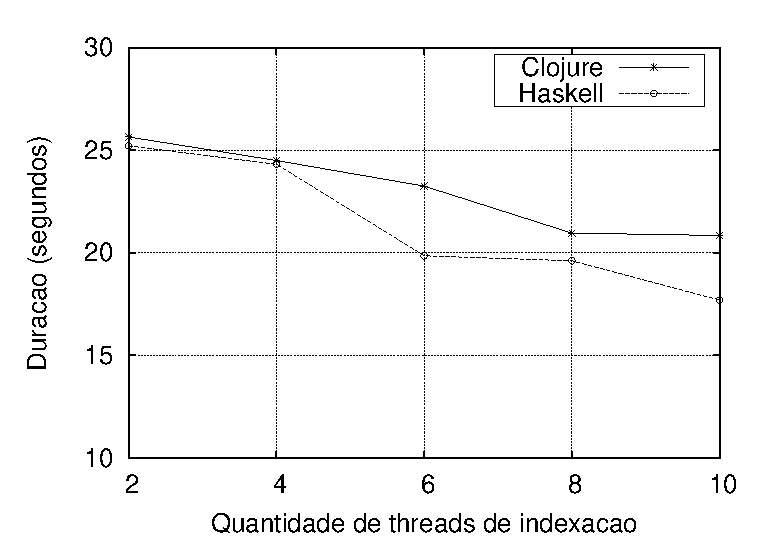
\includegraphics[scale=0.85]{imagens/clojure-haskell.eps}
 \caption{Gráfico do desempenho das versões paralelas em Clojure e Haskell}
 \label{fig:clj-hs-comp}
\end{figure}

A Figura \ref{fig:clj-hs-comp} mostra um gráfico onde o eixo horizontal representa a quantidade de \emph{threads} passada como argumento para o programa e o eixo vertical a duração em segundos da execução do programa. Cada ponto do gráfico representa a média do tempo de execução obtido a partir de 10 execuções consecutivas do programa calculado por meio do comando \verb|time| do Unix.

Como pode-se perceber, o desempenho de ambas as implementações foi bastante semelhante. As duas implementações se comportaram de maneira escalável durante os experimentos realizados, fazendo com que o aumento do número de \emph{threads} acarretasse em uma melhora do desempenho total do sistema.

\begin{figure}[!h]
 \begin{minipage}{0.5\textwidth}
  \centering
  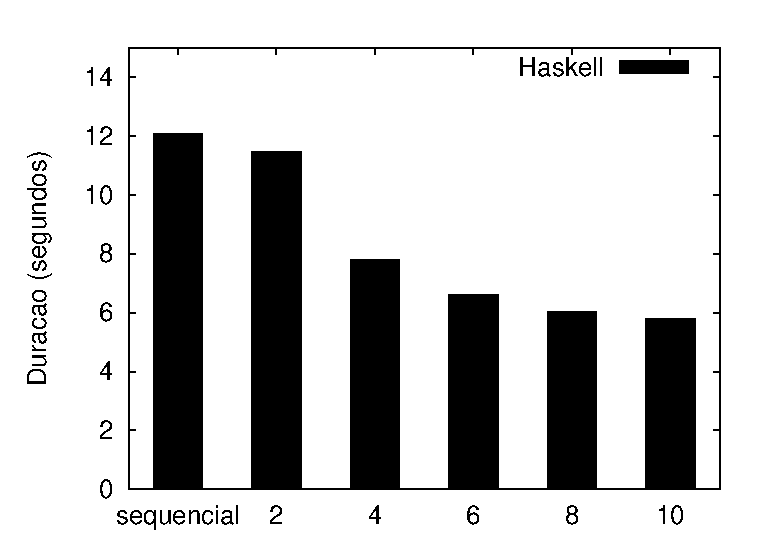
\includegraphics[scale=0.63]{imagens/haskell.eps}
 \end{minipage}
 \begin{minipage}{0.5\textwidth}
  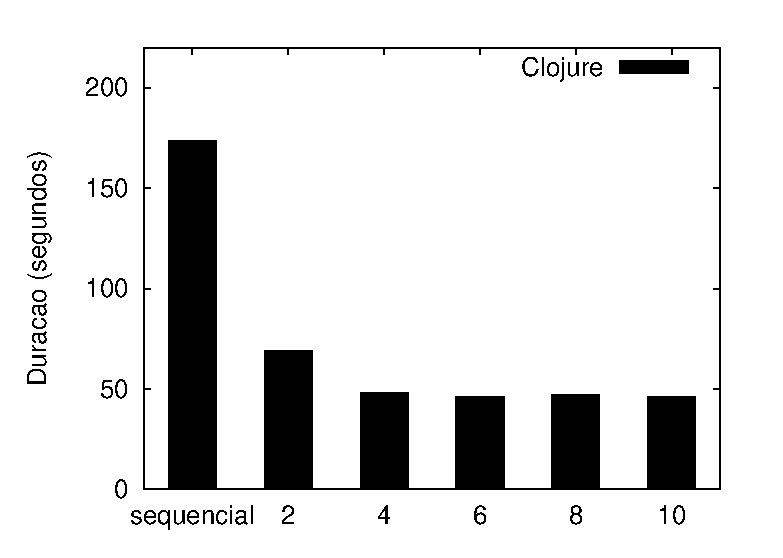
\includegraphics[scale=0.63]{imagens/clojure.eps}
 \end{minipage}
 \caption{Gráficos de comparação de desempenho entre das versões sequenciais e paralelas}
 \label{fig:clj-hs}
\end{figure}

A Figura \ref{fig:clj-hs}, por sua vez, mostra os mesmos dados do gráfico anterior com a adição dos resultados obtidos da execução dos mesmos experimentos com as implementações sequenciais em cada linguagem. Com esses gráficos pode-se notar que o principal objetivo da paralelização do problema foi alcançado já que a versão paralela, em todas as configurações testadas, conseguiu ter desempenho melhor que a versão sequencial.

\begin{figure}[!h]
 \begin{minipage}{0.5\textwidth}
  \centering
  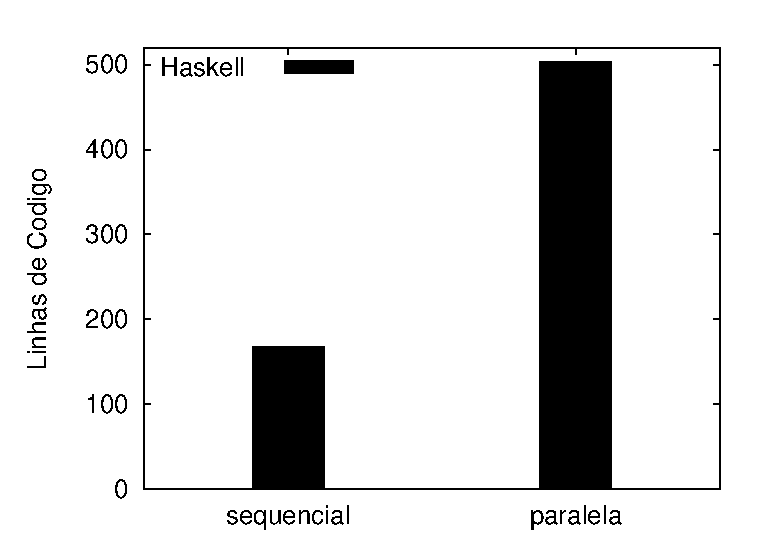
\includegraphics[scale=0.63]{imagens/loc-haskell.eps}
 \end{minipage}
 \begin{minipage}{0.5\textwidth}
  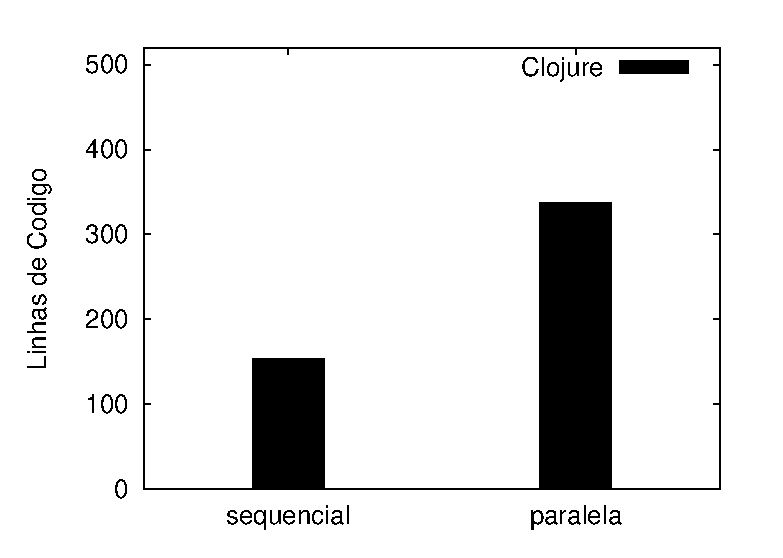
\includegraphics[scale=0.63]{imagens/loc-clojure.eps}
 \end{minipage}
 \caption{Gráficos de comparação da quantidade de linhas de código}
 \label{fig:clj-hs-loc}
\end{figure}

A Figura \ref{fig:clj-hs-loc} mostra o comparativo entre a quantidade de linhas de código total de todas as implementações. Como pode-se perceber, a paralelização implicou em um aumento considerável na quantidade de linhas de código dos projetos. No caso de Clojure, foi um aumento de aproximadamente 120\%, enquanto em Haskell foi um aumento de 200\%. Esse resultado mostra que, de fato, paralelizar um programa implica no aumento da complexidade da solução. Em um ambiente industrial, se faz necessário uma análise mais minuciosa para entender a relação de custo-benefício de se escrever sistemas concorrentes, pois, dependendo do cenário, melhorar o desempenho de um sistema em torno de 40\% ao custo de duplicar ou triplicar a base de código pode ser inaceitável.